
\chapter{The Affixes under investigation}{\label{affixes}}


In this chapter I will describe the five affixes \prefix{un}, negative \prefix{in}, locative \prefix{in}, \prefix{dis} and \suffix{ly} using the relevant morphological and phonological literature. I will discuss their phonological behavior, as well as important morphological, semantic and lexical properties, and compare them with regard to these factors.

Before discussing the affixes, I will give a brief overview of the factors which lead to their inclusion in this study.
The prefixes \is{un-}\prefix{un} and \is{in-}\prefix{in} were included because of two reasons.
First, they are the most prominent examples of \is{morphological gemination}{gemination}/\isi{degemination} given in the literature (see discussion in \sectref{assumptions}).  Second, they are investigated empirically in two previous studies, i.e. a comparison to previous results is possible. 
To investigate an additional prefix, and to also take a look at {gemination} in suffixes, the affixes \is{dis-}\prefix{dis} and \is{-ly}\suffix{ly}  were added to the data set. The choice to include these two affixes was on the one hand due to their comparatively high type \isi{frequency}, which allows for testing type-specific effects on {gemination}, and  on the other due to their phonological and morphological make-up.
The five affixes partly overlap in their characteristics, such as their semantics, their prosodic make-up and their \isi{segmentability}. Importantly, they also show some major differences in their features. This combination of similarities and differences between the affixes makes it possible to test various factors which potentially affect \is{morphological}geminationacross affixes.

In the following, I will describe the formal and structural characteristics of each affix, lay out their phonological and prosodic behavior, and discuss their semantics. Since the literature is often not very specific, or even contradictory when discussing certain aspects of \isi{affixation} (e.g. \isi{stress} pattern or \isi{productivity}), it is often not possible to give a clear-cut description of a certain affix and its behavior. I will remain neutral regarding most of the controversial issues but lay out the different possibilities, as found in the literature.  

After looking at each affix in isolation, I will compare the five affixes with each other. It is of prime importance to look at the differences between the affixes, since these differences lead, according to the theories discussed, to different predictions for their gemination behavior. I will pay special attention to \isi{boundary strength} as it is one of the most important factors for predicting \is{morphological gemination}{gemination}.  
At the end of this section, I will provide some insightful figures regarding the scope of the phenomenon across affixes. In other words, I will lay out how many types with a \is{morphological gemination}{morphological geminate} exist for each affix.

\section{Description of the affixes}

\subsubsection{The prefix \prefix{un}} {\label{description un}}

The affix \is{un-}\prefix{un} is a native prefix which takes native and non-native bases. According to \citet[ 355, 361, 371 ff]{Bauer.2013}, its bases can be verbs, nouns and adjectives. The prefix rarely changes the category of its base and does not take bound roots. It is one of the most productive prefixes in English and has a clearly negative meaning, which varies slightly depending on the base it attaches to. On verbs its meaning is reversive (e.g. \textit{screw} vs. \textit{unscrew}) and sometimes privative (e.g. \textit{dress} vs. \textit{undress}), on adjectives its meaning is contrary or contradicting (e.g. \textit{cool} vs. \textit{uncool}), and on nouns it mostly is privative (e.g. \textit{faith} vs. \textit{unfaith}).
In general, the meaning of \is{un-}\prefix{un}derivatives is very transparent. Only few forms exist in which one cannot deduce a derivative's meaning by adding the negative meaning of \is{un-}\prefix{un} to that of its base (e.g. \textit{unorthodox}).

Turning to the prefix's phonological attributes, \is{un-}\prefix{un} shows what can be called `optional assimilation'. This assimilation affects \is{un-}\prefix{un}derivatives with a base starting in a bilabial (e.g. \textit{unplugged, unbreakable, unmarried}) and \is{un-}\prefix{un}derivatives with a base starting in a velar plosive (e.g. \textit{ungrateful, uncool}).
Before bilabials the prefix-final nasal sometimes is realized as [m]. Before velar plosives the prefixal nasal sometimes is velarized, i.e. realized as [ŋ] (cf. \citealt[5 f]{Hanote.2010}; \citealt[180]{Bauer.2013}; \citealt[125]{Okada.2013}). 
This optional assimilation is not mirrored in \isi{orthography} and, according to \citet[125]{Okada.2013}, is purely phonetic, i.e. not phonological, in nature. \citet[87 f]{Stockwell.2001} explain the optional assimilation of \is{un-}\prefix{un} by a conflict between ``ease of pronunciation" and ``transparency". While the assimilation of the nasal makes pronunciation easier, the transparent nature of the prefix blocks its total assimilation.
Except for one study (\citealt{Hanote.2010}), there is, according to my knowledge, no empirical work on the assimilation of English \is{un-}\prefix{un}. \cite{Hanote.2010} found no systematic pattern with regard to assimilation with \is{un-}\prefix{un}. However, since the authors restricted their study on dictionary data it is questionable how generalizable their results are.  
As \citet[138]{Raffelsiefen.1999}, for example, proposes, assimilation with \is{un-}\prefix{un} might be sensitive to register.  According to her,  assimilation is most likely to occur in fast, \is{conversational speech}{casual speech}. This would mean that dictionary data is not suited to investigate the matter.
To conclude, \is{un-}\prefix{un} sometimes assimilates but the pattern of its assimilation is yet unclear.




Before discussing the \isi{stress} status of \is{un-}\prefix{un}, a general note on prefix \isi{stress} is in order. The \isi{stress} of prefixes is not well researched and observations are mostly anecdotal, i.e. rely on individuals' intuitions rather than on empirical studies. Furthermore, as evidenced in \cite{Videau.2015}, prefixal stress depends on various factors, such as \isi{semantic transparency}, syntactic context and extra-linguistic context. It is yet unclear how these factors interact, i.e. it is unclear how exactly they influence \isi{stress} with prefixes.
Even when leaving contextual influences aside, i.e. when concentrating on lexical \isi{stress} in isolated words, it is quite difficult to determine the \isi{stress} pattern of prefixed words. 

The determination of \isi{stress} for monosyllabic prefixes, such as \is{un-}\prefix{un}, \is{in-}\prefix{in} and \is{dis-}\prefix{dis}, is of special difficulty. When followed by an unstressed syllable, they are, due to prosodic constraints, usually taken to be \is{stress}stressed. Matters are, however, more complicated when the prefix is followed by a \is{stress}stressed syllable. In those cases it is very challenging to determine the relative prominence relations between the prefix and the base-initial syllable, i.e. it is very hard to determine whether the prefix is \is{stress}stressed or not. 
While it is generally assumed that prefixes can bear \isi{stress}, it is unclear how \isi{stress} patterns in those cases. In other words, it is unclear whether the prefix is unstressed, whether it bears primary \isi{stress} or whether it bears secondary \isi{stress}. As discussed in \citet[126]{Okada.2013} for \is{un-}\prefix{un}, \prefix{in} and \textit{non-}, there is variation within prefixes, and this variation ``leads linguists to different descriptions''. 
To summarize, due to difficulties in determining \isi{stress} and the not well researched variation in prefix \isi{stress}, the descriptions of prefixal stress deviate between sources for the prefixes \is{un-}\prefix{un}, \prefix{in} and \is{dis-}\prefix{dis}. %The \isi{stress} pattern of the prefixes is unclear.


The available descriptions of \isi{stress} with \is{un-}\prefix{un} reflect the problems just pointed out. While \citet[4]{Allen.1978} notes that the prefix never bears \isi{stress}, other sources such as \citet[464 f]{Jespersen.1965} and \citet[126]{Okada.2013} state that \is{un-}\prefix{un} is a stress-preserving prefix that may carry \isi{stress}. Similarly in \cite{Wells.2008} \is{un-}\prefix{un} can be \is{stress}stressed. Except for \cite{Allen.1978}, all sources agree that \is{un-}\prefix{un} is \is{stress}stressed if the base-initial syllable of the pertinent derivative is unstressed (e.g. \textit{ˌunconˈventional}\footnote{Throughout this book I will use ˈ to mark primary \is{stress}stressed syllables and ˌ to mark secondary \is{stress}stressed syllables.}).
Assumptions deviate for those cases in which the first syllable of the derivative's base is \is{stress}stressed (e.g. \textit{unˈjust}). \citet[464 f]{Jespersen.1965} notes for these cases that, while in some of the most common \is{un-}\prefix{un}derivatives the prefix is unstressed (e.g. \textit{unˈcommon, unˈhappy}), in most cases the prefix is \is{stress}stressed (e.g. \textit{ˈunˈaided, ˈunˈjust}). 
In \citet[808]{Wells.2008} it is noted that, while generally the prefix may be either \is{stress}stressed or unstressed in those cases, verbs always have a \is{stress}stressed prefix (e.g. \textit{ˌunˈcoil}). Furthermore, it is noted that \is{un-}\prefix{un} ``is unstressed particularly where it is not a true prefix (\textit{unˈwieldy})'' (808). Wells does not give a definition of true prefixhood though, i.e. this statement is quite unclear. Divided or uncertain usage is annotated for some of the \is{un-}\prefix{un}prefixed words with a \is{stress}stressed base-initial syllable (e.g. \textit{\textsubscript{(}ˌ\textsubscript{)}unˈbearable, \textsubscript{(}ˌ\textsubscript{)}unˈleash}). As evidenced in a study by \citet[2 ff]{Hanote.2010}, the assignment of prefixal stress with \is{un-}\prefix{un} in \cite{Wells.2008} does not follow any systematic pattern.
One can thus state that the literature does not provide clear, systematic and empirically-based criteria for \isi{stress} in derivatives with a \is{stress}stressed base-initial syllable. It therefore remains unclear when \is{un-}\prefix{un} is \is{stress}stressed and when it is unstressed. 


One can summarize that \is{un-}\prefix{un} is a very segmentable and very productive prefix. Its meaning is clearly negative and transparent in the vast majority of derivatives. The fact that \is{un-}\prefix{un} only optionally assimilates can be interpreted as a result of its high \isi{segmentability} which blocks total assimilation, and  which hence ensures the prefix's phonological independence from its base. With regard to \isi{stress}, one can state that \is{un-}\prefix{un} can bear \isi{stress} but that the \isi{stress} pattern of the prefix is yet unclear.



\subsubsection{The prefix \prefix{in}} \label{theory:in}

When investigating the prefix \is{in-}\prefix{in}, one must acknowledge the existence of two different \prefix{in}prefixes in English: \is{negative in-}negative \prefix{in} and \is{locative in-}locative \prefix{in}. While the existence of \is{negative in-}negative \prefix{in} is uncontroversial, the idea of \is{locative in-}locative \prefix{in} may not be as straightforward. The reason is that \is{locative in-}locative \prefix{in} often occurs in derivatives with bound roots, such as \textit{inject} or \textit{infuse}. In these words the discrete meaning of \prefix{in}, as well as the discrete meaning of the base, is often unclear. This might lead to the view that locative \textit{in-} is not a prefix but some sort of unit below the word level with  no clear semantic content. This view, however, neglects that \is{locative in-}locative \prefix{in} does indeed have a stable meaning.  

Let us take the standard methodological approach to morphological categories according to which an affix should have an identifiable, stable meaning across different words (cf., for example, \citealt[chapter 5.2.2]{Plag.1999}; \citealt[63 ff]{Stockwell.2001}; \citealt[68]{Schulte.2015}). Under this approach, we would consider \prefix{in} a locative prefix in all those words (and only in those) where the word-initial string \prefix{in} can be assigned some locative meaning and where at the same time the remaining string is also attested outside that word with a stable, identifiable meaning.
Implementing this method, we would be able to assign some locative meaning to the string \prefix{in} in words such as \textit{infuse} `to pour in', \textit{implant} `to plant in' and \textit{import} `to bring in' (\textit{OED online} paraphrases). The remaining strings, i.e. the bases, in these words are all attested (either as words or as bound roots) outside these words with sufficiently similar meaning (cf. \textit{transfuse}, \textit{plant}, \textit{export}). This small sample thus shows that, at least in some words, there is a locative prefix \prefix{in}. 


In this study, all words in which the affix and the base carry a stable meaning are considered as morphologically complex.  Since, complex words with both \prefix{in}prefixes exist, i.e. negative and \is{locative in-}locative \prefix{in}, both types of \is{in-}\prefix{in} are included in the study.  Below I will take a closer look at each type of \prefix{in}.




\subsubsection{Negative \prefix{in} } \label{negative in}

Differently from \prefix{un}, \is{negative in-}negative \prefix{in} is a non-native (or Latinate) prefix that takes non-native bases. It mostly takes adjectives as its base (e.g. \textit{intolerant, immortal}). Only sometimes nouns are taken as its base (e.g. \textit{inexperience}).  In most cases, \is{negative in-}negative \prefix{in} does not change the word class of its derivative.  Usually free bases are found with \is{negative in-}negative \prefix{in} (e.g. \textit{intolerant, impossible}), but in some derivatives bound roots are found (e.g. \textit{inept, innocent}). In these words it is, however, questionable whether \prefix{in} can even be considered a prefix (cf. \citealt[356 f, 611]{Bauer.2013}).

The majority of the literature claims that \is{negative in-}negative \prefix{in} is not productive (cf. \citealt[1688]{Bauer.2002}). A search of hapax legomena in the Corpus of Contemporary American English (\citealt{Davies.20082014}), as carried out by \citet[361] {Bauer.2013}, reveals however that there is indeed a number of new derivatives with negative \textit{in}-. Examples are \textit{immedical, inactual, inconservative} and \textit{inextractable}.  One should note, however, that \is{negative in-}negative \prefix{in} is far less productive than \prefix{un}, which carries similar meaning. Both prefixes denote contrary or contradictory meaning on adjectives.
 Because of these similarities in meaning the prefixes are often treated as rivals. It is often claimed that the existence of a derivative featuring one of the two prefixes blocks the existence of  a derivative with the other. According to this view, the existence of the word *\textit{inhappy}, for example, is blocked by the existence of the word \textit{unhappy} (see, for example,  \citealt[467 ff]{Jespersen.1965}, \citealt[1688 f]{Bauer.2002} and \citealt[377 ff]{Bauer.2013} for discussion).  
As reported by \citet[377]{Bauer.2013}, the idea of rivalry between the two prefixes is, however, invalidated by the existence of derivatives such as \textit{inaccessible} and \textit{unacessible}. There is no noticeable difference in meaning between the two derivatives, and in turn there is no difference in meaning between the two prefixes \is{un-}\prefix{un} and \prefix{in}.
However, while the two prefixes often are identical in meaning, \citet[379]{Bauer.2013}, similar to  \cite{Jespersen.1965} and \cite{Bauer.2002},  note that \prefix{in}derivatives are more often lexicalized than derivatives with \prefix{un}. To summarize, while \is{negative in-}negative \prefix{in} is very similar to \prefix{un} in its meaning, it does not share its high degree of \isi{productivity} and its consistency with regard to \isi{semantic transparency}.

Turning to the phonological features of \is{negative in-}negative \prefix{in}, one must mention its obligatory assimilation. Before a bilabial the prefixal nasal becomes /m/. Before a base-initial lateral the nasal becomes /l/, and before an alveolar rhotic it becomes /r/. Examples are \textit{impossible}, \textit{immortal}, \textit{illogical} and \textit{irregular} (cf. \citealt[1687]{Bauer.2002}; \citealt[359]{Bauer.2013}; \citealt[123 f]{Okada.2013}). This assimilation is also mirrored in \isi{orthography}. 

With regard to \isi{stress}, \prefix{in}, similar to \prefix{un}, is generally assumed to be \is{stress}stressed when followed by an unstressed syllable (cf. \citealt[473]{Jespersen.1965}; \citealt[381, 384]{Wells.2008};  \citealt[183]{Bauer.2013}; \citealt[126]{Okada.2013}). Examples are \textit{ˌinexˈhaustible, ˌindeˈscribable} and \textit{ˌimmeˈmorial}. In those cases \prefix{in} bears secondary \isi{stress}. There are also some derivatives, such as \textit{ˈimpotent} and \textit{ˈimpious}, in which \prefix{in} is primarily \is{stress}stressed. \citet[183]{Bauer.2013} note that while  \isi{stress} with \prefix{in} seems unsystematic in general,  the prefix seems to only bear primary \isi{stress} when the base of the derivative is bound.
In case of a \is{stress}stressed base-initial syllable, \prefix{in} is, in contrast to \prefix{un}, generally taken to be unstressed (cf. \citealt{Wells.2008}; \citealt[183]{Bauer.2013}; \citealt[126]{Okada.2013}). 

We can summarize that, while \is{negative in-}negative \prefix{in} is similar in meaning to \is{un-}\prefix{un}, it is less semantically and phonologically transparent. It is also less productive. Negative \prefix{in} has more bound roots than \is{un-}\prefix{un}, is sometimes semantically opaque, and derivatives are more often lexicalized. The prefix is phonologically more integrated in its base than \is{un-}\prefix{un}. This is indicated by the obligatory assimilation of the prefix. The \isi{stress} pattern of \prefix{in} can also be interpreted as an indicator of its phonological integration. While in some respects the \isi{stress} pattern is similar to the one of \is{un-}\prefix{un}, the prefix, contrary to \is{un-}\prefix{un}, also bears primary \isi{stress} in some cases. Primary \isi{stress} emerges with bound roots and denotes \isi{stress shift}, i.e. in those derivatives the position of primary \isi{stress} has shifted from the base to the prefix. This shows that the boundary between prefix and base is rather weak.\\


\subsubsection{Locative \prefix{in}} \label{locative in}

Locative \prefix{in} differs in interesting respects from \is{negative in-}negative \prefix{in}. Differently from negative \prefix{in}, the origin of \is{locative in-}locative \prefix{in} is twofold. This leads to a prominent distinction in the literature. Traditional approaches differentiate between non-native (or Latinate) \is{locative in-}locative \prefix{in} and native \is{locative in-}locative \prefix{in}.  While the first one is commonly analyzed as a prefix which takes non-native bases, the second is often analyzed as a locative particle (cf. \citealt[497 ff]{Jespersen.1965}; \citealt[115,163 f]{Marchand.1969}; \citealt[1685]{Bauer.2002}). Examples are given below:

\begin{exe}
	\ex non-native locative \prefix{in}: \hspace{0.7cm} \textit{inject, immigrate, impress}
	\ex native locative \prefix{in}: \hspace{1.4cm} \textit{inborn, inbreed, indoors}
\end{exe}

\cite{Bauer.2013} also make a distinction between the two different cases but regard both types of \is{locative in-}locative \prefix{in} as prefixes. Since the authors only discuss productive prefixes, and since they consider non-native \is{locative in-}locative \prefix{in} unproductive,  only native \prefix{in} is discussed in their work. It is said to be a productive prefix that attaches to nouns, adjectives and verbs. It takes native and non-native bases (\citealt[334, 340]{Bauer.2013}).
 
 It is generally assumed that the two types of \is{locative in-}locative \prefix{in} differ in their type of base, their \isi{productivity} and in the degree of phonological assimilation they display. While the non-native prefix is believed to mostly take non-native bases (see \citealt[499]{Jespersen.1965}), native \prefix{in} also attaches to native bases (see \citealt[334]{Bauer.2013}). While non-native \is{locative in-}locative \prefix{in} is not productive, the native form is believed to be productive. With regard to phonological assimilation, non-native \is{locative in-}locative \prefix{in} undergoes the same obligatory assimilation as negative \prefix{in}, while native \is{locative in-}locative \prefix{in} is described as only optionally assimilating (see \citealt[499]{Jespersen.1965}; \citealt[335]{Bauer.2013}). The common assumption thus seems to be that non-native \is{locative in-}locative \prefix{in} is phonologically and semantically less transparent than native \is{locative in-}locative \prefix{in}. There are, however, no empirical studies investigating whether these criteria mirror the distinction between the two types of \is{locative in-}locative \prefix{in}. 
 

It is not easy to distinguish between native and non-native \is{locative in-}locative \prefix{in}. This problem is  already discussed in early works such as \citet[499]{Jespersen.1965} and \citet[164]{Marchand.1969}. The semantics of both types of \is{locative in-}locative \prefix{in} overlap to a high degree. Both prefixes denote a locative meaning, which is formulated as ‘into, in, within; on, upon; towards, against’ in the \textit{OED online}\nocite{OED.2013}. The \textit{OED} further mentions that 

\begin{displayquote}
``[s]ince \prefix{in} prefix 1 [non-native \prefix{in}] and \textit{ in-} prefix 2 [native \prefix{in}] are identical in form, and to a great extent in sense, they come in later use to be felt as one and the same prefix; and it is this resulting prefix which appears in many words of later formation.''
\end{displayquote}

It is thus suggested that, while \is{locative in-}locative \prefix{in} has two origins, the distinction between the two formerly distinct types of \is{locative in-}locative \prefix{in} is no longer clear. This is in line with the observation that the criteria used to distinguish native from non-native \is{locative in-}locative \prefix{in} are rather blurry. 
In this study, I will not explicitly distinguish between the two types of \is{locative in-}locative \prefix{in}. I will, however, account for differences in \isi{semantic transparency}, phonological make-up and type of base in my studies. I therefore will be able to implicitly differentiate between more \is{decomposability}decomposable and less \is{decomposability}decomposable \is{locative in-}locative \prefix{in}derivatives, which in turn, according the literature, may mirror the distinction between native and non-native \is{locative in-}locative \prefix{in}.

With regard to \isi{stress}, the literature is mostly silent about a distinctive \isi{stress} pattern for \is{locative in-}locative \prefix{in}. Except for \citet[384]{Wells.2008}, who notes that \prefix{in} is ``generally \is{stress}stressed only
(i) if meaning `in' rather than `not''', there are no explicit mentions about the \isi{stress} pattern of \is{locative in-}locative \prefix{in}. While, according to \cite{Wells.2008}, \is{locative in-}locative \prefix{in} is \is{stress}stressed and \is{negative in-}negative \prefix{in} is not, there are also sources which state that \is{negative in-}negative \prefix{in} can be \is{stress}stressed (see description of negative \prefix{in} above). It is thus unclear whether there is a systematic difference between the \isi{stress} pattern of locative and negative \prefix{in}. One could venture the idea that \is{locative in-}locative \prefix{in}, due to its assumingly higher \isi{frequency} of bound roots, more often bears primary \isi{stress} than negative \prefix{in}. This would fit in with \citeauthor{Wells.2008}'s statement. It, however, is an assumption that calls for empirical evidence.

To summarize, \is{locative in-}locative \prefix{in} is of two different origins which makes it rather difficult to make clear statements about the prefix. It seems that it occurs quite frequently with bound bases, is often semantically opaque and less productive than negative \prefix{in}. In other words, \is{locative in-}locative \prefix{in} seems to have a weaker morphological boundary than negative \prefix{in} and \is{un-}\prefix{un}. This impression is, however, to be tested empirically.

 
\subsubsection{The prefix \prefix{dis}}

The prefix \is{dis-}\prefix{dis} is a non-native (or Latinate) prefix that takes mostly native bases. Occasionally non-native bases are found in \is{dis-}\prefix{dis}derivatives (e.g. in the word \textit{disbelief}). The prefix takes mostly verbs and nouns as its base, sometimes adjectives. It is rarely category-changing and mostly takes words as its bases (see \citealt[481]{Jespersen.1965}; \citealt[158 ff]{Marchand.1969}; \citealt[355, 357]{Bauer.2013}).
According to \citet[358]{Bauer.2013}, the few \is{dis-}\prefix{dis}derivatives with bound roots, such as \textit{distort}, came to English as borrowings. Furthermore, the authors state that these borrowed words differ in their phonological structure from the other \is{dis-}\prefix{dis}words (e.g. in their \isi{stress} pattern).


As negative \prefix{in} and \prefix{un}, the prefix \is{dis-}\prefix{dis} denotes negativity.  With adjectives \is{dis-}\prefix{dis} is, similar to \is{un-}\prefix{un} and \prefix{in}, contrary or contradictory (e.g. \textit{dishonest}). It is only in this category that \is{dis-}\prefix{dis} is productive (see \citealt[358]{Bauer.2013}). With nominal bases \is{dis-}\prefix{dis} is privative (e.g. \textit{disbelief}). With verbs it often is privative or reversative (e.g. \textit{disconnect} or \textit{disarm})  (see \citealt[372, 375]{Bauer.2013}).
Because of the similarities in meaning between \is{un-}\prefix{un}, \is{negative in-}negative \prefix{in} and \is{dis-}\prefix{dis}, the discussion of affix rivalry can be extended to the prefix \is{dis-}\prefix{dis}. 
As with \prefix{un} and \prefix{in}, there is, however, no evidence for the blocking of one derivative by the existence of another. This is indicated by the co-existence of \prefix{un} and \is{dis-}\prefix{dis}derivatives with the same base and identical meaning (see \citealt[380]{Bauer.2013}). Examples are \textit{unarm} / \textit{disarm} and \textit{uncharge} / \textit{discharge}. 
\citet[380]{Bauer.2013} note that semantic differences between \is{un-}\prefix{un} and \is{dis-}\prefix{dis} are restricted to specific derivatives and are due to lexicalization. The prefix \is{dis-}\prefix{dis} is more often lexicalized than the prefix \is{un-}\prefix{un} (e.g. \textit{unbar} `remove the bar' vs. \textit{disbar} `remove from the bar, i.e. to be disqualified from practicing law').

Different from \prefix{in}, there is no systematic assimilation of the prefix \is{dis-}\prefix{dis}. However, as mentioned by \citet[480]{Jespersen.1965}, in some \is{dis-}\prefix{dis}derivatives the prefix-final fricative has assimilated to its base-initial vowel by becoming voiced (e.g in the words \textit{disease} and \textit{dissolve}). Note that in these words assimilation goes together with \isi{resyllabification}. \citet[158]{Marchand.1969} claims that this assimilation with \is{dis-}\prefix{dis} can only be found in monomorphemic words, such as in the word \textit{disaster}. However, while most of the \is{dis-}\prefix{dis}words with a voiced fricative are indeed simplex, at least some can be categorized as complex using to the methodology described above (e.g. \textit{disease} and \textit{dissolve}). Note that in these assimilated words the meaning of the derivative cannot be deduced from the meaning of its parts, i.e. they are semantically opaque. Hence, in these words \isi{semantic opacity} goes together with phonological opacity.

The \isi{stress} pattern of \is{dis-}\prefix{dis}prefixed words is similar to the \isi{stress} pattern of \prefix{in} prefixed words. In derivatives with an unstressed base-initial syllable \is{dis-}\prefix{dis} is assumed to be \is{stress}stressed (e.g. \textit{ˌdisalˈlow, ˌdisenˈdow}). In derivatives with bases starting in a \is{stress}stressed syllable, such as \textit{disˈown}, the prefix is usually unstressed (see \citealt[479 f]{Jespersen.1965}; \citealt[183]{Bauer.2013}). There are also some \is{dis-}\prefix{dis}derivatives which bear primary \isi{stress} on the prefix (e.g. \textit{ˈdisparate, ˈdiscount, ˈdissipate}). 
\citet[183, 360]{Bauer.2013} state, however, that primary \isi{stress} with \is{dis-}\prefix{dis} is very rare and mostly restricted to semantically opaque derivatives with bound roots. On a more general note, the authors furthermore note that \isi{stress} with \is{dis-}\prefix{dis} does not seem to follow a systematic pattern. In \citet[223]{Wells.2008} it is stated that \is{dis-}\prefix{dis} is  ``\is{stress}stressed when followed by an unstressed syllable, and often even when not''. This statement also mirrors that there does not seem to be a systematic and accurate description of the \isi{stress} behavior of \is{dis-}\prefix{dis}.


All in all, \is{dis-}\prefix{dis} is less productive and less transparent than \prefix{un}. Some derivatives are semantically opaque and feature bound roots.  There is no systematic phonological assimilation. Only in a few derivatives assimilation can be found. These derivatives are, however, often regarded as simplex. As stated by \citet[440]{Bauer.2013}, in most derivatives \is{dis-}\prefix{dis} behaves like a prosodically independent word, i.e. there is no phonological integration of the prefix with its base. There are, however, a few cases in which \is{dis-}\prefix{dis} bears primary \isi{stress} (e.g. \textit{discount}), as well as a few derivatives with an assimilated fricative (e.g. \textit{disease}). This indicates that for some \is{dis-}\prefix{dis}derivatives there is some phonological integration of the prefix with its base.\\

\subsubsection{The suffix \suffix{ly}}\label{ly}

The fourth affix investigated in this study is the native suffix \is{-ly}\suffix{ly}. There are two different types of \is{-ly}\suffix{ly} in English, adjectival \is{-ly}\suffix{ly} as in \textit{friendly} and adverbial \is{-ly}\suffix{ly} as in \textit{coolly}. In this study, I will concentrate on adverbial \is{-ly}\suffix{ly}.

Adverbial \is{-ly}\suffix{ly} has been a quite frequent topic of discussion in the morphological literature (see for example \citealt{Zwicky.1995}; \citealt{Plag.2003}; \citealt{Giegerich.2012}; \citealt{Bauer.2013}). Debates revolve around the question of whether the suffix is inflectional or derivational. 
The main argument for the derivational status of adverbial \is{-ly}\suffix{ly} is that the suffix is category changing, i.e. it takes adjectives as its base and turns them into adverbs. However, in this context the question of whether adverbs and adjectives should be seen as two distinct syntactic categories must be raised. If one does not adhere to the adjective-adverb distinction, the category-changing argument is no longer valid (cf. \citealt[195]{Plag.2003}; \citealt{Giegerich.2012}).
	
There are various arguments for the inflectional status of \is{-ly}\suffix{ly}. First, adverbial \is{-ly}\suffix{ly}, in contrast to the majority of derivational suffixes, cannot be followed by other derivational suffixes. In some cases it is even preceded by an inflectional suffix (e.g. in the word \textit{interestingly}) (cf. \citealt{Giegerich.2012}).
Second, \is{-ly}\suffix{ly} does not denote a clear lexical meaning (cf. \citealt[195]{Plag.2003}; \citealt{Giegerich.2012}; \citealt[324]{Bauer.2013}). The suffix itself just expresses manner, means, duration, {frequency} and temporal relations. It follows that the meaning of \is{-ly}\suffix{ly}-derivatives is mostly determined by the meaning of their base and not by the meaning of the suffix (see \citealt[326 f]{Bauer.2013}). 
Third, the suffix \is{-ly}\suffix{ly} is, similar to inflectional suffixes, very transparent and productive. \citet[196]{Plag.2003} mentions that only a few semantically opaque \is{-ly}\suffix{ly}-words exist. Examples are \textit{hardly} and \textit{shortly}. 
The suffix is very productive and can more or less freely attach to any adjective. The only restriction to its \isi{productivity}, mentioned in \citet[334]{Bauer.2013}, is its reluctance to attach to bases already ending in \is{-ly}\suffix{ly}.
While its high \isi{productivity} and the lack of a clear semantic meaning might indeed suggest that \is{-ly}\suffix{ly} is inflectional, \citet[324]{Bauer.2013} point out that there are also other English derivational suffixes with similar features (e.g. \textit{-al} and \textit{-ment}) whose derivational status is not doubted. 
 
To summarize the discussion about the derivational status of adverbial \is{-ly}\suffix{ly}, there are arguments for both assumptions, i.e. in some respects adverbial \is{-ly}\suffix{ly} behaves like an inflectional suffix and in some it behaves like a derivational suffix. As pointed out by \citet[196]{Plag.2003} the distinction between inflection and derivation might not be categorical, and \is{-ly}\suffix{ly} might be an example of an affix which lies in between.

Turning to phonology, some \is{-ly}\suffix{ly}-derivatives, such as  \textit{markedly} and \textit{amazedly}, display base allomorphy. In those derivatives an epenthetic vowel is inserted between base and suffix to meet the prosodic requirement of \is{-ly}\suffix{ly}. As reported by \citet[172]{Bauer.2013}, \is{-ly}\suffix{ly} requires bases with more than one syllable to form a  trochee before the suffix. If the base does not meet this requirement, vowel epenthesis, i.e. base allomorphy, is used change the prosodic structure of the base. The suffix itself does, however, not display any allomorphy. 

\citet[163]{Bauer.2013} report that some \is{-ly}\suffix{ly}-derivatives display \isi{resyllabification}. They provide the word \textit{frailly} as the only example. Note that the {morphological geminate} /ll/ in this example is assumed to be realized as a single syllable-initial consonant, i.e. the authors assume \isi{degemination}. This demonstrates that \isi{resyllabification} is closely connected to {gemination}, and that it should, if possible, be taken into account when investigating {gemination}.
However, \isi{resyllabification} is very difficult to investigate. \citet[168]{Bauer.2013} attribute  this difficulty to the variability found in \isi{resyllabification}. Furthermore, syllable boundaries are very difficult to determine and empirical evidence is needed to make valid statements. Up to now this empirical evidence is lacking, and therefore, no statement about \isi{resyllabification} with \is{-ly}\suffix{ly} can be made.
With regard to \isi{stress}, one can state that the suffix is never \is{stress}stressed and that it does not cause \isi{stress} shifts in its base (cf. \citealt[1670]{Bauer.2002}; \citealt[323]{Bauer.2013}).

To summarize, \is{-ly}\suffix{ly} is a very productive and \is{semantic transparency}{semantically transparent} suffix. Because of its regularity, formal properties and its rather weak semantic contribution, it is often argued to be inflectional. The suffix is, however, category-changing and therefore usually categorized as derivational. It is unstressed, sometimes causes allomorphy in its base and might \is{resyllabification}{resyllabify}.


\section{Comparison of the affixes}\label{comparison affixes}

The analysis above has revealed that the affixes \is{un-}\prefix{un}, \is{negative in-}negative \prefix{in}, \is{locative in-}locative \prefix{in}, \is{dis-}\prefix{dis} and \is{-ly}\suffix{ly} are characterized by different phonological, morphological and semantic properties. These differences lead to differences in \isi{boundary strength}, which in turn lead to different predictions for \isi{gemination}.  Because of this relation of \isi{boundary strength} and predictions for \isi{gemination}, it is necessary to compare the affixes with regard to their \isi{boundary strength}. 

The notion of \isi{boundary strength} generally refers to the morphological boundary which separates the affix from its base. This strength can, however, be defined in different ways. One can look at it from a prosodic point of view by asking to which degree an affix is phonologically integrated in its base. Alternatively, one can look at it from a lexical point of view, taking factors such as \isi{semantic transparency} and \isi{productivity} into account. In the following comparison I will take different viewpoints, i.e. I will compare the affixes and their {boundary strengths} from a phonological/prosodic point of view and  from a lexical point of view. In addition to the term \isi{boundary strength}, I will use the terms \newterm{decomposability} and \newterm{segmentability}. While I will use the term \isi{decomposability} when talking about derivatives, I will use the term \isi{segmentability} when talking about affixes. The stronger a boundary, the more \is{decomposability}decomposable is the derivative and the more segmentable is the affix.







\begin{sidewaystable} 
	
	
	\caption{The affixes under investigation: a comparison}
	\label{tbl:The affixes under investigation: a comparison}
	\resizebox{\textwidth}{!}{%
		
		
		\begin{tabular}{llllll}
			\lsptoprule
			%\midrule\\
			                  & \textit{\textbf{un-}}                                                                 &\textbf{negative} \textit{\textbf{in-}}                                                            & \textbf{locative} \textit{\textbf{in-}}                                          & \textit{\textbf{dis-}}                                                                    & \textit{\textbf{-ly}}                                                                           \\
			\midrule\\
			\textbf{Assimilation}      & 
			\begin{tabular}[c]{@{}l@{}}non-obligatory \\ affix assimilation\end{tabular}          & \begin{tabular}[c]{@{}l@{}}obligatory\\ affix assimlation\end{tabular}                    & \begin{tabular}[c]{@{}l@{}}mostly obligatory\\ affix assimilation\end{tabular} & 
			\begin{tabular}[c]{@{}l@{}}no\\ assimilation\end{tabular}                                 & \begin{tabular}[c]{@{}l@{}}\\ base assimilation\end{tabular}     \\
			
			\textbf{Resyllabification} & no        & no           & no    & no     & possibly      \\
			
			\textbf{Stress}   & possible & possible& possible& possible                                                                                  & never {stressed}    \vspace{0.5cm }\\
			
			\textbf{Type of Base} & free bases & mostly free bases & frequently bound bases& mostly free bases & free bases    \\
			
			\textbf{Semantics} &clearly negative & clearly negative &locative  &clearly negative & no clear meaning \\
				
		 \textbf{Semantic Transparency} & transparent &mostly transparent& mostly opaque & mostly transparent &transparent  \\
	
			\textbf{Productivity}      & very productive   & productive & rarely productive  & productive & very productive    \\
				\lspbottomrule                                                                                
		\end{tabular}%
	}
	
\end{sidewaystable}


\tabref{tbl:The affixes under investigation: a comparison} summarizes the characteristics of each affix as described in the previous sections. Looking at phonological and prosodic factors, it is striking that \is{-ly}\suffix{ly} is different from all other affixes in the set. It is never \is{stress}stressed, claimed to \is{resyllabification}resyllabify and may lead to base assimilation. All other affixes in the set may be \is{stress}stressed and do not \is{resyllabification}resyllabify. For those affixes which undergo assimilation, the assimilation always affects the affix, i.e. not the base. One major reason for the differences between \is{-ly}\suffix{ly} and the other affixes might of course be the fact that \is{-ly}\suffix{ly} is the only suffix in the set. With regard to \isi{prosodic boundary} strength, one can assume that the possible \isi{resyllabification} and the fact that \is{-ly}\suffix{ly} is always unstressed hint at a rather weak boundary between base and suffix.

Comparing the four prefixes with each other, the two \prefix{in}prefixes show the most integration with their base. This is indicated by their obligatory assimilation. Even though there might be some derivatives with \is{locative in-}locative \prefix{in} which do not undergo assimilation (some derivatives with native \is{locative in-}locative \prefix{in}), the number of these derivatives is assumed to be very small. It is therefore assumed that \is{locative in-}locative \prefix{in} assimilates to a similar degree as \is{negative in-}negative \prefix{in}. The prefixes \is{dis-}\prefix{dis} and \is{un-}\prefix{un} integrate less with their base. For \is{dis-}\prefix{dis} only a few derivatives assimilate. For \is{un-}\prefix{un} assimilation is optional. 
A valid comparison of \isi{stress} with the four prefixes is difficult to make. This is due to the general problems with determining prefixal stress.  However, based on the descriptions above, it seems that while primary \isi{stress} is possible on \prefix{in} and \is{dis-}\prefix{dis}, it is not on \is{un-}\prefix{un}. Prefixal primary \isi{stress} can be regarded as part of a prefix's phonological integration with the base. Only in derivatives with a rather weak \isi{prosodic boundary} the base's \isi{stress} pattern can be changed in \isi{affixation}, i.e. primary \isi{stress} can be shifted from the base to the affix. In other words, prefixes with primary \isi{stress} are less segmentable and feature a weaker boundary. Thus, with regard to \isi{stress}, \is{un-}\prefix{un}, which is never primarily \is{stress}stressed, is more segmentable than the other three prefixes.

Overall the following picture emerges. The strongest \isi{prosodic boundary} can be found in \is{un-}\prefix{un}derivatives, followed by \is{dis-}\prefix{dis}derivatives. Both \prefix{in}prefixes have a rather weak \isi{prosodic boundary}. Because of general differences between prefixes and suffixes a comparison of \is{-ly}\suffix{ly} with the other affixes is difficult. However, since \is{-ly}\suffix{ly} features a rather weak \isi{prosodic boundary}, its prosodic \isi{segmentability} can be assumed to be comparable to the one of \prefix{in}, which also features a weak \isi{prosodic boundary}.



Turning to lexical factors, the prefix \is{un-}\prefix{un} is the most transparent and most segmentable affix. In other words, it has the strongest boundary. This is indicated by its high \isi{productivity}, its clear semantics and the fact that it takes only words as its base. The suffix \is{-ly}\suffix{ly} is similar to \is{un-}\prefix{un} in its \isi{productivity}, transparency and the type of base it takes. A very important difference is, however, that \is{-ly}\suffix{ly} does not denote a clear lexical meaning. Therefore, the boundary between base and affix is assumed to be weaker for \is{-ly}\suffix{ly} than for  \is{un-}\prefix{un}. 
Negative \prefix{in} and \is{dis-}\prefix{dis} are very similar with regard to their lexical attributes. Both of them are productive, have a preference for words as their base, have mostly transparent derivatives and denote a clear lexical meaning. They are assumed to be less segmentable than \is{un-}\prefix{un}, which is even more transparent and productive. The comparison to \is{-ly}\suffix{ly} is difficult. On the one hand, \is{-ly}\suffix{ly} is more productive and more transparent than \is{negative in-}negative \prefix{in} and \is{dis-}\prefix{dis}, on the other, \is{-ly}\suffix{ly}, in contrast to \is{negative in-}negative \prefix{in} and \is{dis-}\prefix{dis}, does not denote a clear meaning. Whether the two prefixes or the suffix have a stronger boundary therefore depends on how one ranks the importance of a clear lexical meaning for determining \isi{boundary strength}. Locative \prefix{in} has the weakest boundary of the four prefixes. Its meaning is mostly opaque, it is rarely productive and very often takes bound roots. In contrast to \is{-ly}\suffix{ly}, \is{locative in-}locative \prefix{in} does, however, denote a clear lexical meaning when \is{semantic transparency}{semantically transparent}.


\figref{fig:Segmentability hierarchies of  affixes} summarizes the comparison of affixes by displaying \isi{segmentability} hierarchies. In these \isi{segmentability} hierarchies the affixes are sorted by their \isi{boundary strength}. Since \isi{boundary strength} can be defined in different ways, three hierarchies are displayed. The first one orders the affixes by \isi{prosodic boundary} strength (\newterm{Prosodic Hierarchy}), the second and the third by lexical \isi{boundary strength} (\newterm{Semantic Hierarchy}, \newterm{Non-Semantic Hierarchy}). The difference between the {Semantic Hierarchy} and the {Non-Semantic Hierarchy} is that in the {Semantic Hierarchy}  lexical meaning is regarded as a more important criterion for \isi{boundary strength} than \isi{productivity}, \isi{semantic transparency} and type of base. The opposite is assumed in the {Non-Semantic Hierarchy}. This leads to different positions of the suffix \is{-ly}\suffix{ly}. While in the {Semantic Hierarchy} \is{-ly}\suffix{ly} is ranked as the least segmentable affix, in the {Non-Semantic Hierarchy} it is positioned between \is{dis-}\prefix{dis}, \is{negative in-}negative \prefix{in} and \is{un-}\prefix{un}.

Overall one can see similar patterns in all hierarchies. This shows that prosodic and lexical \isi{boundary strength} cannot be regarded as two independent concepts but that they rather go hand in hand. For example, in all hierarchies \is{un-}\prefix{un} is very segmentable and \is{locative in-}locative \prefix{in} is rather less segmentable, i.e. features a rather weak boundary. However, there are also differences between the hierarchies. Especially the ranking of the suffix \is{-ly}\suffix{ly} highly depends on which criteria one applies to determine \isi{boundary strength}.


\begin{figure*}
		
	
	\begin{tabularx}{\textwidth}{lll}
		
		& \textbf{Segmentability}&	\textbf{Additional 	}  		  \\
		
			&	\textbf{hierarchy	}	&		\textbf{assumption }  	  \\		
		\midrule\\
		\textbf{Prosodic}	&	\prefix{un} > \prefix{dis} > \{\prefix{in}\textsubscript{\textsc{Neg}}, \prefix{in}\textsubscript{\textsc{Loc}}, \suffix{ly}\}	 & 		  \\ 
		\textbf{Hierarchy}&&\\
		\\
		\textbf{Semantic} & \prefix{un} > \{\prefix{dis}, \prefix{in}\textsubscript{\textsc{Neg}}\}>  \prefix{in}\textsubscript{\textsc{Loc}} > \suffix{ly}& lexical meaning over pro-	 		  \\	
		\textbf{Hierarchy}	& & ductivity, transparency and 	 		  \\	
		& & type of base			 		  \\	
		\\
		\textbf{Non-Semantic}	&  	\prefix{un} > \suffix{ly} > \{\prefix{dis}, \prefix{in}\textsubscript{\textsc{Neg}}\}>  \prefix{in}\textsubscript{\textsc{Loc}}&		 {productivity}, transparency			   \\	
			\textbf{Hierarchy}& & and  type of base	over   \\	
		& & lexical meaning		  		  \\	
			\midrule \\						
	\end{tabularx}
	
	\caption{Segmentability hierarchies of  affixes}
	\label{fig:Segmentability hierarchies of  affixes} 
	
\end{figure*}

There are two important things to note with regard to the hierarchies just proposed. First, they are  based on  theoretical assumptions found in the morphological literature on affixes. These assumptions are only partly supported by empirical evidence, and it is therefore necessary to empirically test whether they are borne out by the data. This will be done in this book.
Second, the hierarchies proposed are based on categorical distinctions. In other words, they assume very similar behavior across the derivatives of one affix. This means that predictions on \is{morphological gemination}{gemination} based on these hierarchies can only predict the behavior of all derivatives of an affix, not the behavior of individual words. Some of the theoretical approaches discussed in the next sections are categorical in nature. For these approaches I will return to the \isi{segmentability} hierarchies in order to make predictions about \is{morphological gemination}{gemination}. For gradient approaches, i.e. approaches that  do not assume the uniform behavior of the derivatives of a certain affix,  the \isi{segmentability} hierarchies are of less relevance.


\section{Scope of gemination across affixes} \label{scope of gemination}

Let us now have a look at the scope of \is{morphological gemination}{gemination} for each affix. An easy way to get an idea of how many types with morphological {geminates} exist for each affix is conducting a corpus study. Using the query tool \newterm{Coquery} (\citealt{Kunter.2016}), I searched the DVD version of the {Corpus of Contemporary American English (\isi{COCA})} (\citealt{Davies.20082014}) for all \is{un-}\prefix{un}, \prefix{in}, \is{dis-}\prefix{dis} and \is{-ly}\suffix{ly}-affixed words with an orthographic double consonant at the morphological boundary. With more than 520 million words \isi{COCA} is one of the largest available corpora for English. It can therefore be assumed that the number of types found in the corpus is representative of the actual number of types.

I searched for morphological \is{morphological gemination}{geminates} by querying orthographic strings. For prefixes I searched for the orthographic string the prefix is made of followed by the last segment of the prefix, i.e. <unn> for \is{un-}\prefix{un},  <inn> for \is{in-}\prefix{in} and  <diss> for \is{dis-}\prefix{dis}. Note that I also conducted a search for the allomorphs \is{im-}/ɪm/, /ɪr/ and /ɪl/ of \prefix{in}, i.e. I also searched for the orthographic strings  <imm>, <irr> and <ill>.  For the suffix \is{-ly}\suffix{ly}, I searched for the sequence <lly>.  I then checked the morphological status of the words found using the {CELEX} database (\citealt{Baayen.1995}) and the {English Lexicon Project (ELP)} (\citealt{Balota.2007}). All words which, according to at least one of the two databases, featured the affix in question were included in the count. 
Note that, due to the fact that the two databases do not feature all existing affixed types, and that not all existing types with a \is{morphological gemination}{morphological geminate} are attested in \isi{COCA}, the count presented here is not exhaustive. Furthermore, morphological \is{morphological gemination}{geminates} which are not represented by the sequence of two identical orthographic segments (e.g. \textit{solely, unknown}) are not taken into consideration. Nevertheless, the count conducted is useful to get a general impression of the scope of \isi{morphological gemination} across the affixes.
 
 \figref{fig:morphological geminates for each affix} shows a bar plot displaying the number of types of morphological \is{morphological gemination}{geminates} for each affix. Each bar represents one affix. The number of types is given next to each bar. The bar for the prefix \prefix{in}  represents the number of types with all four \is{allomorphy}allomorphs of \prefix{in}, i.e. /ɪn/, /ɪm/, /ɪr/ and /ɪl/. 
 
\begin{figure*}  
	
	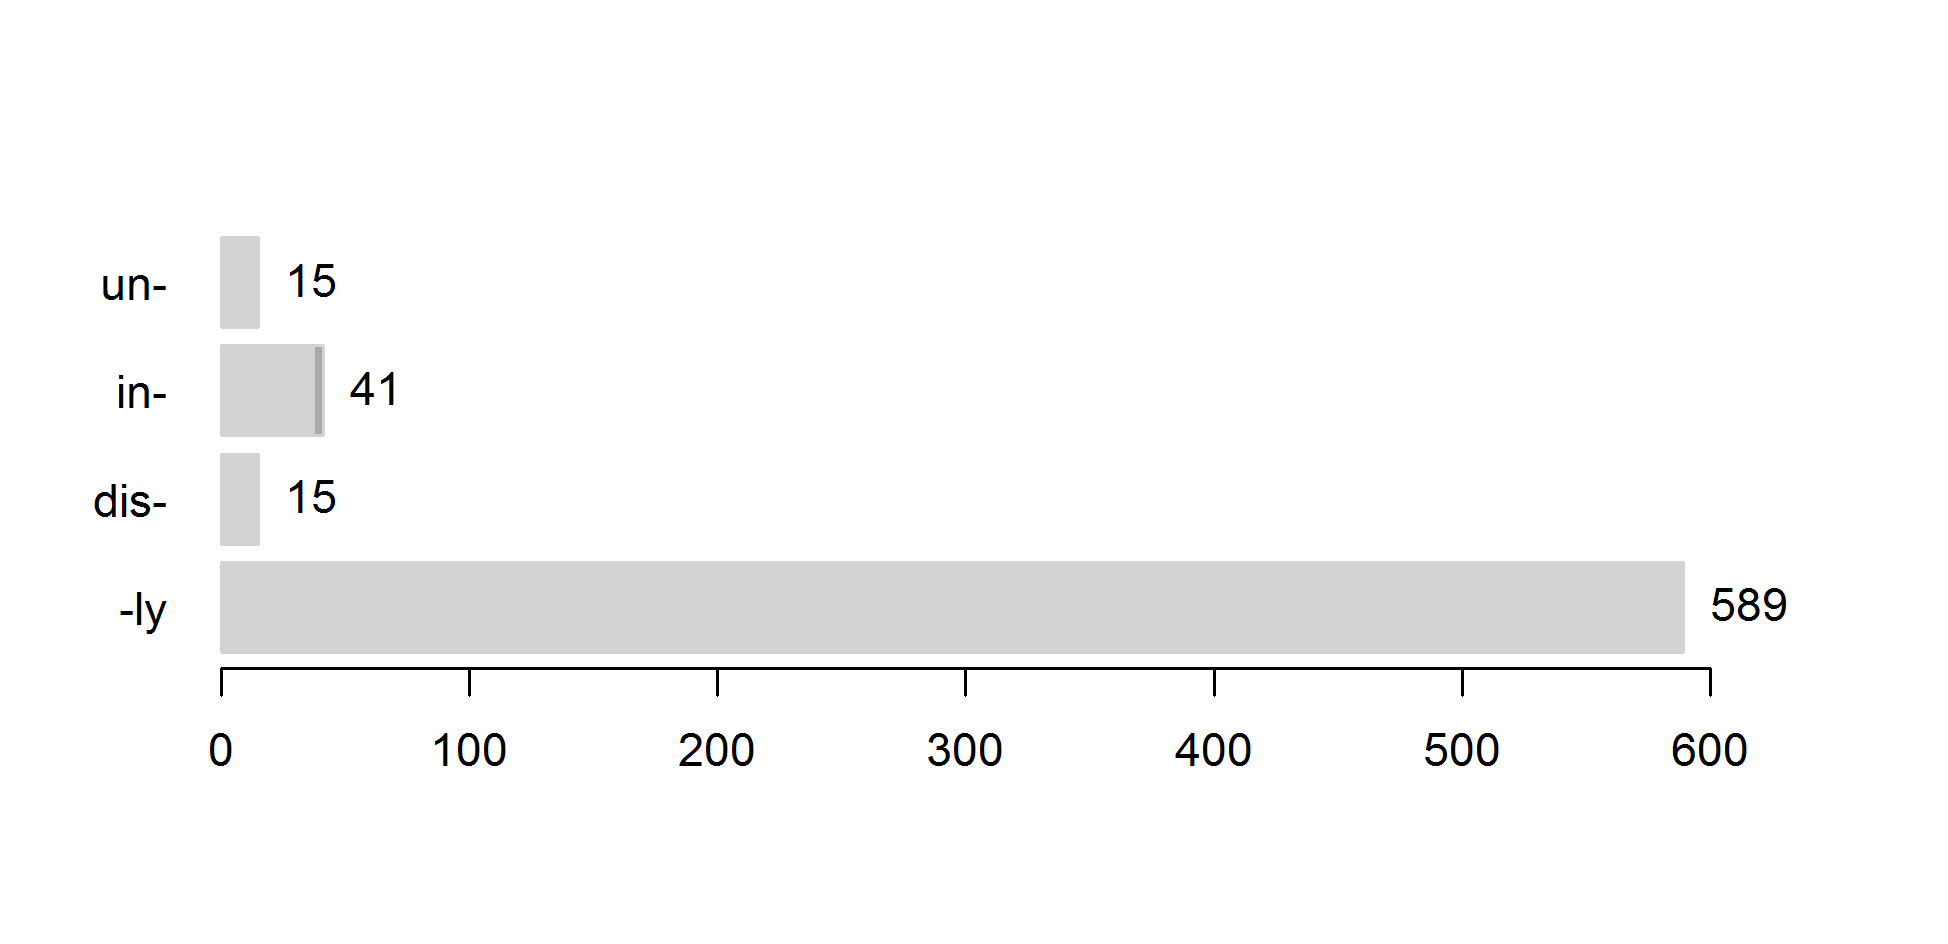
\includegraphics[scale=0.75]{images/Theory/NumberOfMorphGemAffixes.png}
 
	\caption{ Number of types with morphological geminates for each affix}
	\label{fig:morphological geminates for each affix}
\end{figure*}

A comparison of the affixes reveals that while there are quite a lot of types with morphological \isi{geminates} for the suffix \is{-ly}\suffix{ly}, the number of types is much smaller for all of the prefixes. In other words, there are not many \is{un-}\prefix{un}, \prefix{in} and \is{dis-}\prefix{dis}prefixed words with a \isi{morphological geminate}. Especially the number of morphological \isi{geminates} with \is{un-}\prefix{un} and \is{dis-}\prefix{dis} is very small and might raise methodological problems with regard to the investigation of some of the factors possibly influencing \isi{gemination}. Some variables, such as \isi{frequencies}, might not show enough variation to reliably be investigated. I will return to these issues in the pertinent sections of this book.

For the prefix \is{in-}\prefix{in}, the number of attested types with morphological \isi{geminates} is much higher than for the prefixes \is{un-}\prefix{un} and \is{dis-}\prefix{dis}. However, out of the 105 attested types only one features the allomorph /ɪn/ (e.g. \textit{innumerable}). 33 types start with the allomorph\is{im-} /ɪm/ (e.g. \textit{immortal}), 51 with /ɪr/ (e.g. \textit{irregular}), and 20 with /ɪl/ (e.g. \textit{illogical}). 
This distribution has important consequences for the investigation of the prefix. Since the number of types in /ɪn/ is so limited, my investigation of \is{morphological gemination}gemination with \is{in-}\prefix{in} will mainly focus on the allomorph /ɪm/, for which more types exist. This is, as discussed in \sectref{previous empirical work}, in line with previous empirical work on \is{morphological gemination}gemination with \prefix{in}.
The investigation of /ɪr/  and /ɪl/ is not reasonable as derivatives with these allomorphs always feature a \is{morphological gemination}{morphological geminate}, i.e. there are no derivatives with /ɪr/  and /ɪl/ which feature a singleton consonant at their morphological boundary. This makes a comparison of the duration of a phonological double with a phonological singleton impossible.
